% !TEX root = ../my-thesis.tex
%

\chapter{Analysis of Geospatial Health Data}
\label{sec:geodata}
Healthcare data provides information for detecting public health problems and reacting adequately when they occur. With this information, prevention and control of a multitude of health conditions including infectious diseases, non-communicable diseases, injuries and health-related behaviours can be achieved. To analyse and interpret health data, the process involves a wide variety of system designs, analytical methods, modes of presentation and interpretive uses \autocite[][]{teutsch2000principles}. Descriptive methods generally form the basis of routine reporting of surveillance data. Rather than focusing on observed patterns in the data, these may attempt to compare the relative occurrence of health outcomes in different subgroups. More specific hypotheses can be explored using inferential methods. The aim of these methods is to draw statistical inferences about patterns or outcomes of health. \\
There is increasing availability of geo-referenced health data, population data and satellite images of environmental factors that influence levels of disease activity. The development of geographic information systems (GIS) and address geocoding software has facilitated the conduct of studies on spatial and spatio-temporal variations in disease. \\
A broad range of spatial and spatio-temporal methods exist for disease surveillance, including methods for disease mapping, clustering and geographic correlation studies. These methods can be used to identify areas of high risk, risk factors, evaluate spatial variations in temporal trends, measure excess disease risk near a suspected source and detect outbreaks at an early stage.
\clearpage
\section{Geographic Data}
In spatial statistics, two fundamental types of geographic data exist, namely \textit{vector data} and \textit{raster data}. In the vector data model, the world is represented by points, lines and polygons with discrete, well-defined boundaries, which tends to result in high accuracy. Raster data, on the other hand, divides the surface into cells of uniform size, and raster datasets are used as the basis for background images in web mapping. \\
Determining which data type to use depends on the domain of the application. Vector data dominates in the social sciences because human settlements typically have discrete boundaries, while raster data are commonly used in many environmental sciences because they are based on remote sensing data. Naturally, there is some overlap and both types can be used together or one form can be converted into the other \autocite[][]{lovelace2019geocomputation}.
\subsection{Vector Data}
The geographic vector data model is based on points located within a \textit{coordinate reference system} (CRS), in which points either represent self-standing features or form more complex geometric shapes, i.e. lines and polygons. Using this system, Trondheim can be represented by the coordinates $\left(10.4, 63.4\right)$, meaning $10.4$ degrees east of the prime meridian and $63.4$ degrees north of the equator. It could also be written as $\left(1157722.70, 9199010.75\right)$, which is the position of Trondheim using the Web Mercator projection, the de facto standard for web mapping applications. More is said about CRS later, but for now it is sufficient to know that it is possible to display coordinates in various ways. An example of a CRS is shown in Figure~\ref{fig:globe}.

\subsubsection{Different Types of Vector Data}
As mentioned earlier, there are different types of vector data. There are 17 different geometry types in the standard \textit{simple features}, but there are seven core types that can be used in most analysis software. These types are visualized in Figure~\ref{fig:sf}. Simple Features was developed by the Open Geospatial Consortium and is an open, standardized, hierarchical data model that represents a wide range of geometry types. The use of this data model ensures that scientific work can be transferred to other institutions, e.g. when importing from and exporting to spatial databases \autocite[][]{lovelace2019geocomputation}. \clearpage
\begin{figure}[H]
   \centering
       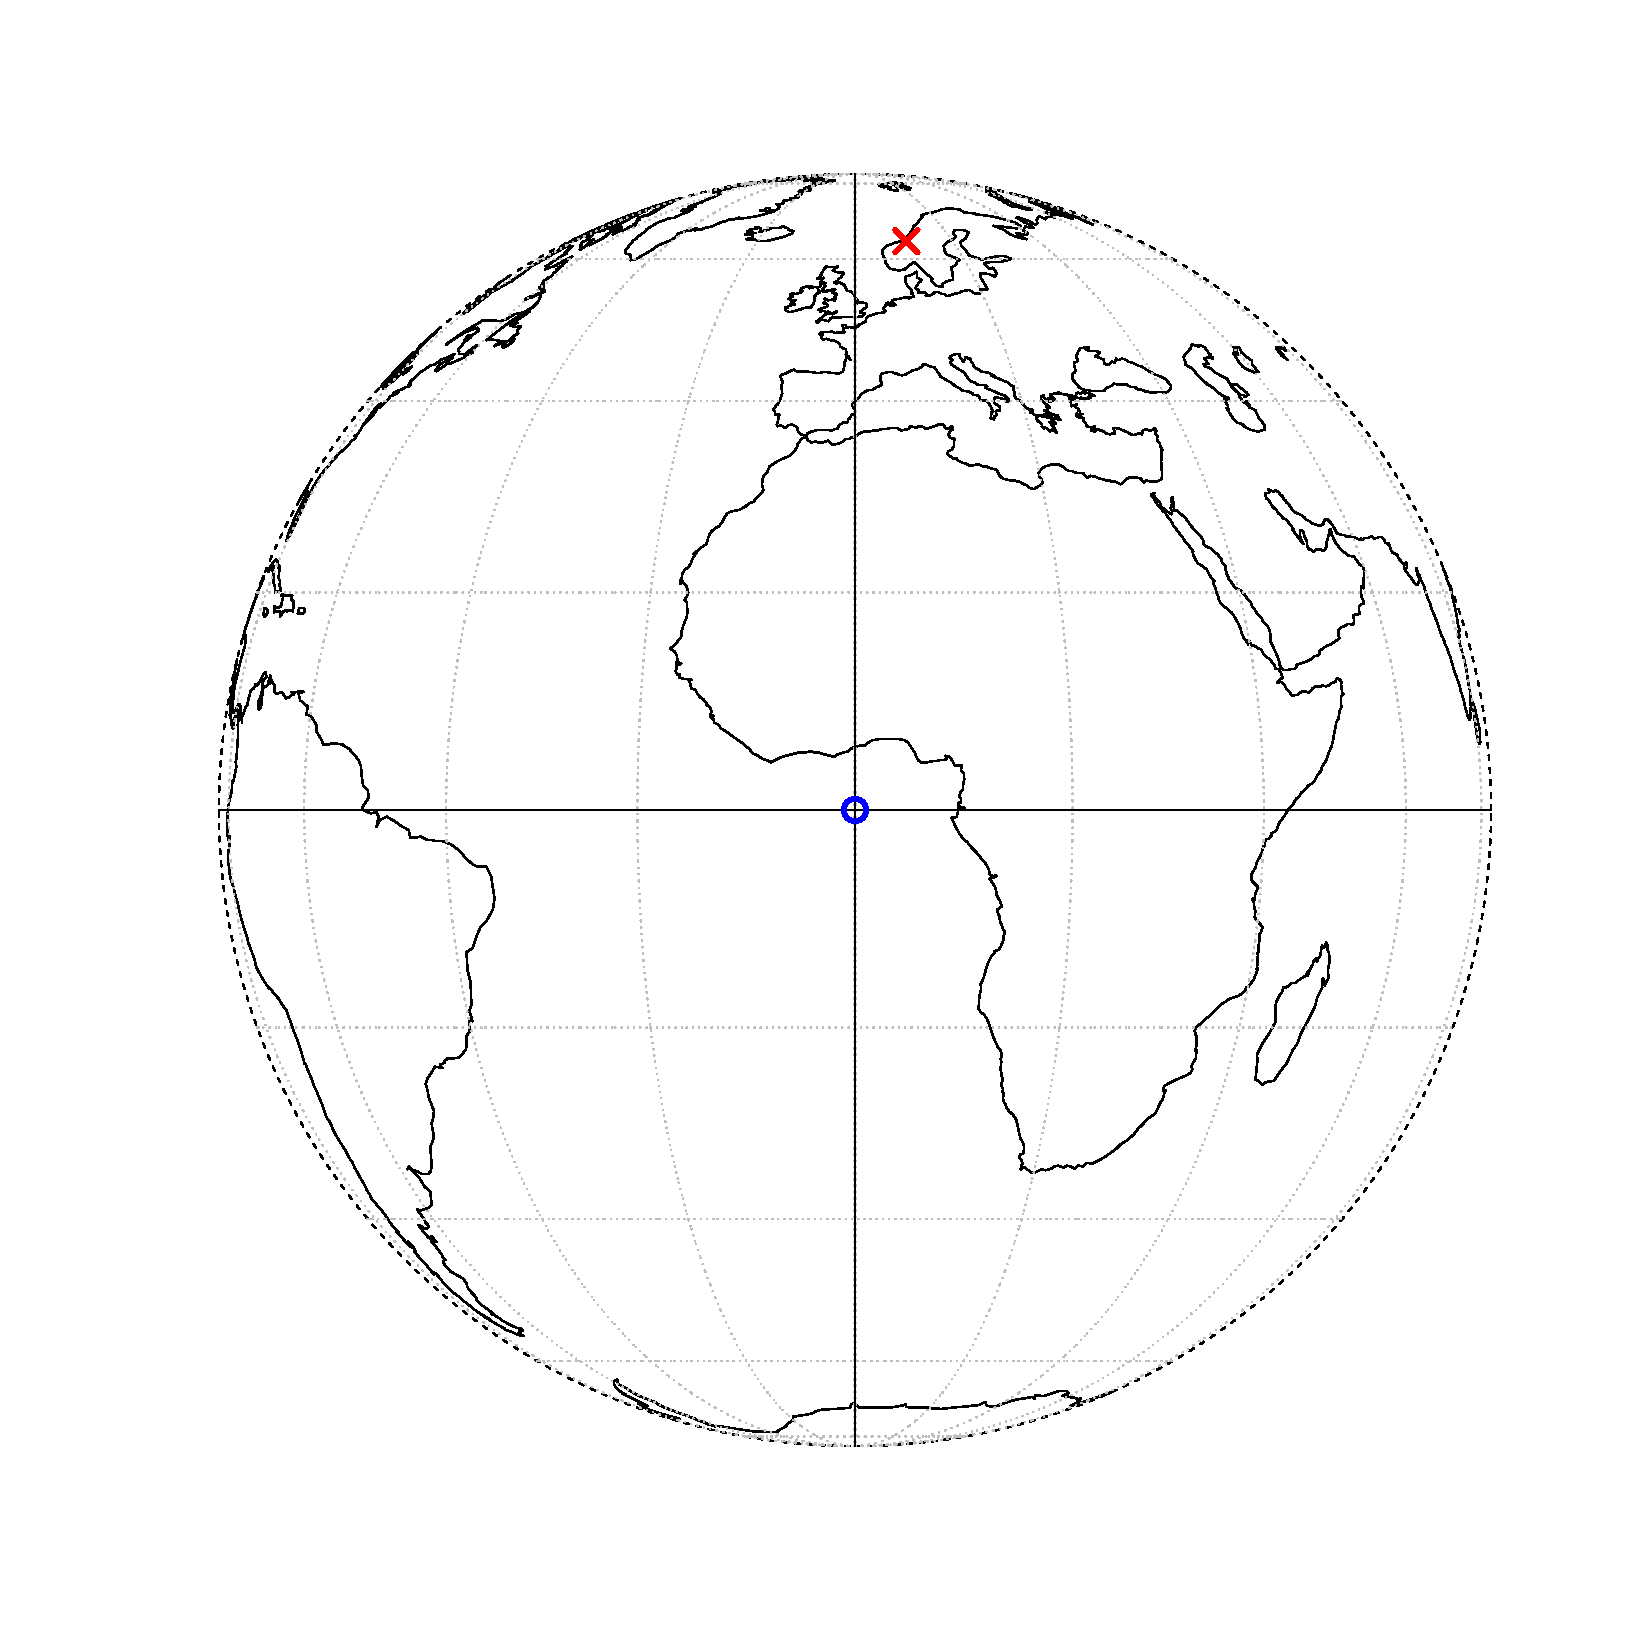
\includegraphics[page=1,width=0.7\textwidth]{globe.pdf}
 \caption{A geographic CRS with an origin at 0° longitude and latitude. The red X denotes the location of Trondheim.}
 \label{fig:globe}
\end{figure}
\begin{figure}[H]
   \centering
       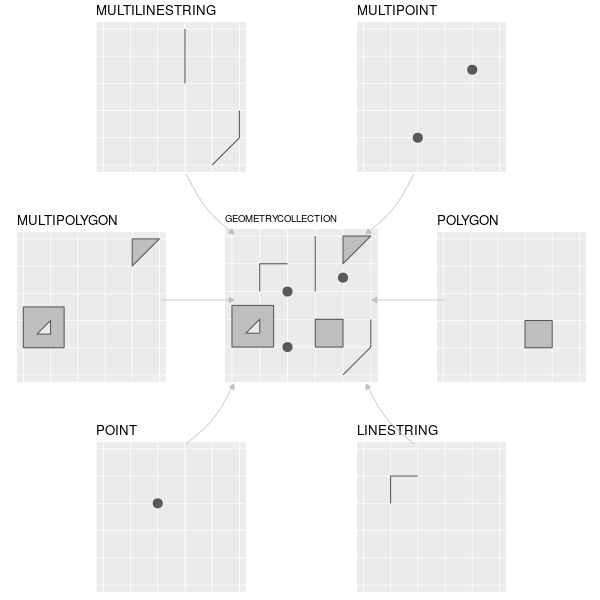
\includegraphics[width=0.7\textwidth]{sf-classes.png}
 \caption{The most commonly used simple feature types.}
 \label{fig:sf}
\end{figure}
\subsection{Raster Data}
The geographic raster data model consists in most cases of a raster header and a matrix representing uniformly distributed cells/pixels. The raster header defines the CRS, the origin (starting point) and the extent. Since the number of columns and rows and the resolution of the cell size are stored in the extent, starting from the origin, it is easy to access and change each cell by its ID or by specifying the row and column number. In this type of representation, the coordinates of the four vertices of each cell are not explicitly stored, instead only the origin is stored. This speeds up data processing and makes it more efficient, but each raster layer can only contain a single value, which can be either numeric or categorical. Typically, raster maps are used to represent continuous features such as elevation or temperature, but categorical variables such as soil or land cover can be represented as well, as shown in Figure~\ref{fig:raster} \autocite[][]{lovelace2019geocomputation}.
\begin{figure}[H]
   \centering
       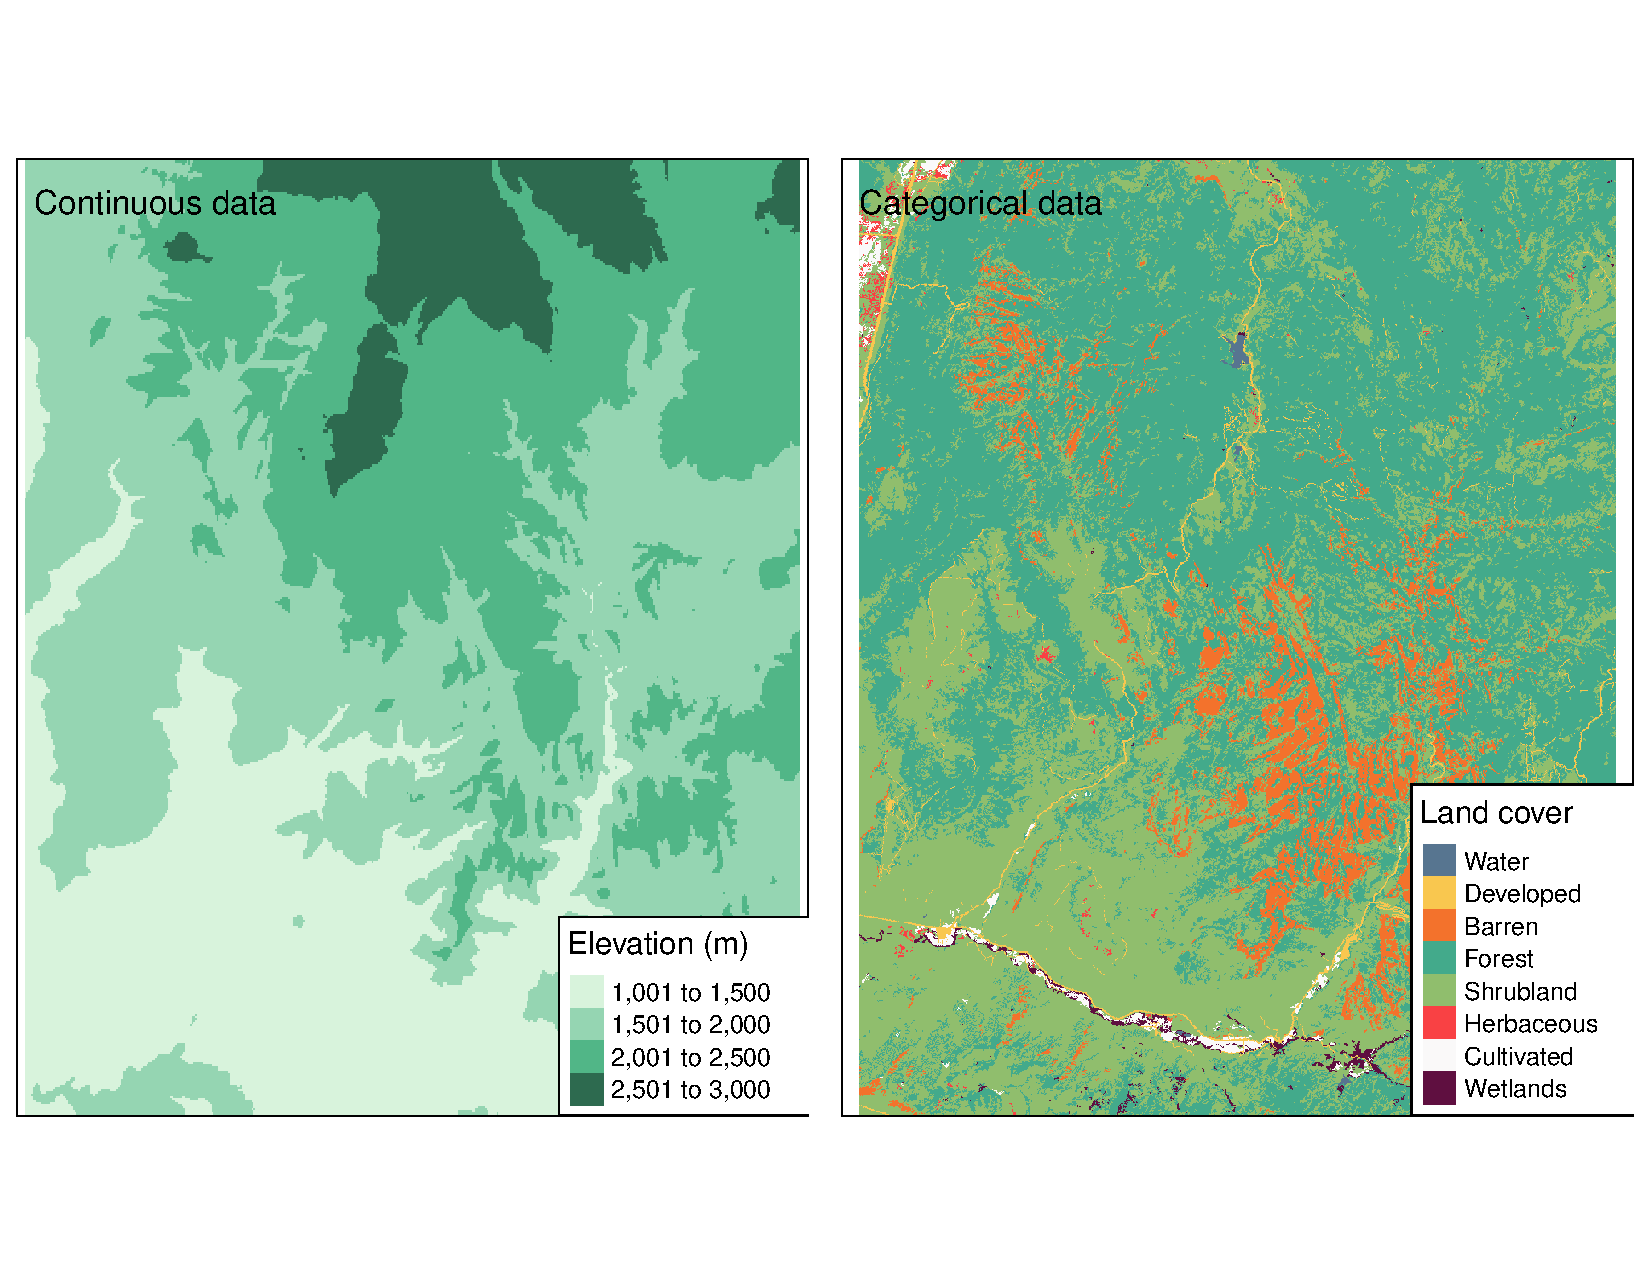
\includegraphics[page=1,width=\textwidth]{raster.pdf}
 \caption{An example of continuous and categorical raster data}
 \label{fig:raster}
\end{figure}
\clearpage
\subsection{Coordinate Reference Systems}
A common denominator of vector and raster data are that both use the coordinate reference system (CRS), which defines how spatial elements relate to the surface of the Earth. The CRS can be either geographic or projected.
\subsubsection{Geographic Coordinate Systems}
Geographic coordinate systems use two values, \textit{longitude} and \textit{latitude}, to identify any location on Earth. Longitude is defined as the east-west location at an angular distance from the prime meridian plane, while latitude is the angular distance north or south of the equator. Consequently, distances in geographic CRS are not measured in metres. \\
The Earth's surface is typically represented in geographical coordinate systems by a spherical or ellipsoidal surface. The former assumes that the Earth is a perfect sphere of a certain radius, which has the advantage of being a simplistic model, but is associated with inaccuracies owing to the fact that the Earth is not a sphere. Ellipsoidal models are defined by the equatorial radius and the polar radius, providing a better model since the equatorial radius is approximately 11.5 km longer than the polar radius.\\
The \textit{datum} is a broader component of CRS that contains information about which ellipsoid to use and the exact relationship between Cartesian coordinates and the location on the Earth's surface. The notation \textit{proj4string} is used to store these additional details. It allows for local variations of the Earth's surface, such as large mountain ranges, to be taken into account in local CRS. Datum can again be divided into two categories, \textit{local} and \textit{geocentric}, the difference being that in the local datum the ellipsoidal surface is shifted to match the surface at a particular location, whereas in the geocentric datum the centre of gravity of the Earth is the centre and the accuracy of the projections is not optimized for any particular location \autocite[][]{lovelace2019geocomputation}.
\subsubsection{Projected Coordinate Systems}
Projected CRS are based on Cartesian coordinates on an implicitly flat surface and have an origin, $x$ and $y$ axes, and a linear unit of measurement, metres for instance. They are based on geographic CRS and rely on map projections to convert between the three-dimensional surface of the Earth and the east/north values ($x$ and $y$) in a projected CRS.\\
This transition always entails some distortion, skewing some properties of the Earth's surface, such as area, direction, distance and shape. Generally, the name of a projection is based on a property it preserves, e.g. equal area projection preserves area, equidistant projection preserves distance and conformal projection preserves local shape. \\
Again, subgroups exist in projection coordinate systems, \textit{conic}, \textit{cylindrical} and \textit{planar} projections. In a conic projection, the Earth's surface is projected onto a cone along one or two tangent lines. Along these lines the distortions are minimized and increase with the distance to the lines. The projection is therefore best suited for maps of mid-latitude areas. Cylindrical projections map the surface onto a cylinder. These types of projections can be created by touching the surface of the Earth along one or two tangent lines. They are often used to map the entire Earth. A planar projection projects data onto a flat surface that touches the globe at a point or along a tangent line, and is typically used in mapping polar projections \autocite[][]{lovelace2019geocomputation}.
\clearpage
\section{Modeling and Visualizing Health Data}
After collecting and cleaning all the data needed to analyse a research question, the next step is the analysis itself. This analysis may involve visualizing the data at hand, for example by visualizing the neighbourhood structure of spatial areas or simply by plotting the locations of all points of interest on a base map. When deciding whether to model spatial dependence, Moran's I \autocite[][]{moran1950notes} can be used to construct a test for spatial correlation between different spatial entities. The standardized incidence ratio (SIR) is a method used to examine the incidence in a small area, such as a municipality. These two methods are presented in Section~\ref{sec:moran} and Section~\ref{sec:sir}. If there is a spatial correlation, it is useful to model this spatial effect using models for risk assessment in spatial areas. The way this is done is introduced in Section~\ref{sec:spatial}. If data are available over a longer period of time and some variables change their values over time or a temporal trend is present, it may be useful to model the spatial and temporal effect by using spatio-temporal models, which are introduced in Section~\ref{sec:spatiotemporal}.
\subsection{Areal Data}
Areal or lattice data are the result of segmenting a fixed domain into a finite number of sub-regions where results are aggregated, e.g. the number of infections with a specific disease in districts or the number of overweight people in provinces. Often the aim of disease risk models is to assess the risk within the same areas for which data are available. This can be done with a simple measure such as the \textit{standardized incidence ratio} (SIR) or by using a Bayesian hierarchical model, which allows information to be drawn from neighbouring areas and incorporates covariates, thereby smoothing and reducing extreme values. 
\subsubsection{Spatial Neighbourhood Matrices}
Spatial or proximity matrices are useful for exploratory analysis of area data. Let $w_{ij}$ denote the $\left(i,j\right)$ element of a \textit{spatial neighbourhood matrix} $\pmb{W}$. $w_{ij}$ connects the two areas in some spatial way. The neighbourhood structure over the complete study region is defined by $\pmb{W}$, and the elements of the matrix can be considered as weights. \clearpage The closer $j$ is to $i$, the more weight is associated with it. The simplest neighbourhood definition is given by the binary matrix
\begin{equation}
    w_{ij}=\begin{cases}
    1 & \hbox{ if regions } i $\hbox{ and }$ j \hbox{ share a border} \\
    0 & \hbox{ else.}
    \end{cases}
\end{equation}
In Figure~\ref{fig:neighbour}, the number of shared borders of each canton in Switzerland are mapped.
\begin{figure}[H]
   \centering
       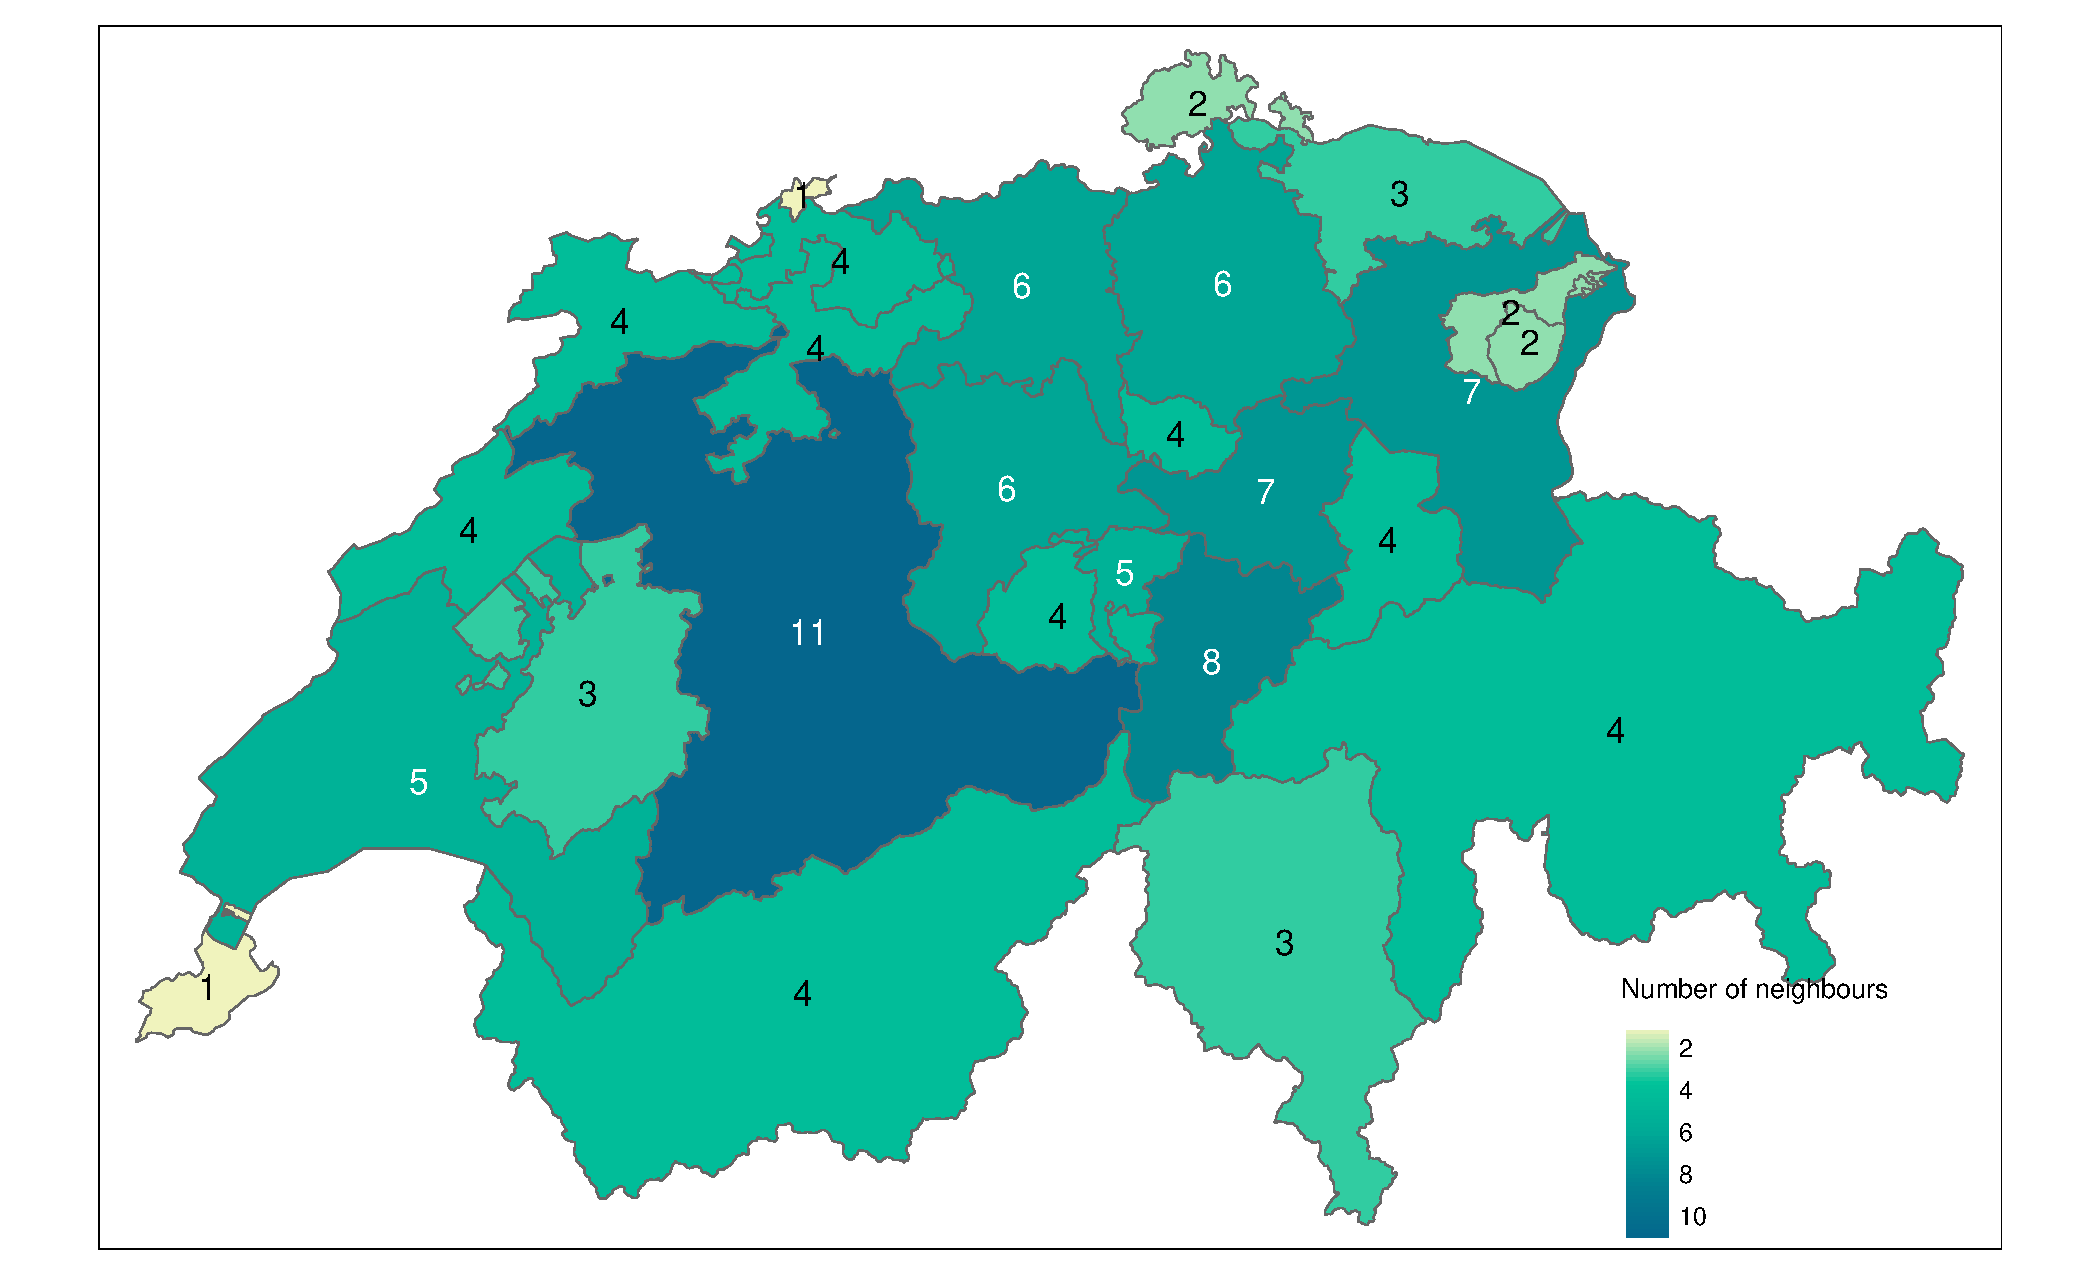
\includegraphics[page=1,width=\textwidth]{neighbours.pdf}
 \caption{The number of shared borders of cantons in Switzerland}
 \label{fig:neighbour}
\end{figure}
\subsubsection{Moran's I}\label{sec:moran}
Moran's I is a measure of spatial autocorrelation developed by Patrick Moran. Spatial autocorrelation is characterized by a correlation in a signal between close locations in space. Spatial autocorrelation is inherently more complex than one-dimensional autocorrelation due to the fact that spatial correlation is multidimensional (i.e. 2 or 3 spatial dimensions) and multi-directional. The formula for Moran's I is given by
\begin{equation}
    I = \frac{n}{\sum_{i=1}^n\sum_{j=1}^nw_{ij}}\frac{\sum_{i=1}^n\sum_{j=1}^nw_{ij}\left(x_i-\overline{x}\right)\left(x_j-\overline{x}\right)}{\sum_{i=1}^n\left(x_i-\overline{x}\right)^2},
\end{equation}
with $n$ denoting the number of spatial units indexed by $i$ and $j$, $x$ the parameter of interest and $\pmb{w}$ a spatial neighbourhood matrix. \clearpage
Using Moran's I, a test for spatial autocorrelation can be constructed with the following hypotheses:
\begin{align}
    H_0:\hbox{ No spatial autocorrelation} \hbox{ vs. }  H_1:\hbox{ Spatial autocorrelation}.
\end{align}
Under $H_0$ the expected value is given by
\begin{equation}
    \mathbb{E}\left[I\right]=\frac{-1}{n-1}.
\end{equation}
As $n$ approaches infinity, the expected value therefore approaches 0.
The significance of Moran's I can be assessed using the $p$-value and a $z$-score. The $z$-score statistic for Moran's I is calculated as follows:
\begin{equation}
    z=\frac{I-\mathbb{E}\left[I\right]}{\sqrt{\hbox{Var}\left(I\right)}}.
\end{equation}
If the returned $p$ value is statistically significant, the null hypothesis can be rejected \autocite[][]{moran1950notes}.
\subsubsection{Standardised Incidence Ratio}\label{sec:sir}
A basic measure of disease risk is the \textit{standardized incidence ratio}, which yields an estimate in each of the areas that form a partition of the study region. It is defined as the ratio of observed counts to expected counts
\begin{equation}\label{eq:sir}
    \hbox{SIR}_i = \frac{Y_i}{E_i}.
\end{equation}
$E_i$ represents the sum of the expected number of cases of a given area $i$ that behave according to the way the standard population behaves. It is calculated using indirect standardization as
\begin{equation}
    E_i=\sum_{j=1}^mr_j^{(s)}n_j^{(i)},
\end{equation}
with $r_j^{(s)}$ the rate in stratum $j$ in the standard population and $n_j^{(i)}$ the population in stratum $j$ of area $i$. If the stratum information is unavailable, the expected counts can be calculated as follows
\begin{equation*}
    E_i = r^{(s)}n^{(i)},
\end{equation*}
where $r^{(s)}$ denotes the rate in the standard population and $n^{(i)}$ is the population of area $i$. If the standardized incidence rate is greater than 1, area $i$ has a higher risk than expected from the standard population, while for $\hbox{SIR}_i = 1$ the risk is the same and for $\hbox{SIR}_i < 1$ it is lower than expected. The ratio is called the standardized mortality ratio when applied to mortality data \autocite[][]{rioux_grandbastien_astagneau_2006}.
\subsubsection{Spatial Small Area Disease Risk Estimation}\label{sec:spatial}
While SIRs may prove useful in some situations, in areas with low population sizes or rare diseases, expected counts may be low, making SIRs insufficiently reliable for reporting. It is therefore preferable to assess disease risk using models that allow information to be borrowed from neighbouring areas and incorporate information from covariates, thus smoothing or shrinking extreme values due to small sample sizes \autocite[][]{gelfand2010handbook}. \\
The observed counts $Y_i$ in area $i$ are typically modelled with a Poisson distribution with mean $E_i\theta_i$, where $E_i$ is the expected counts and $\theta_i$ denotes the relative risk in area $i$. The logarithm of the relative risk is expressed as the total of the intercept and the random effects. $\theta_i$ quantifies whether area $i$ has a higher $\left(\theta_i >1\right)$ or lower $\left(\theta_i <1\right)$ risk than the average risk in the standard population. If the risk of an area $i$ is half the average risk, $\theta_i = 0.5$. The general model for spatial data is formulated as follows:
\begin{align}
    Y_i&\sim\hbox{Po}\left(E_i\theta_i\right), \hspace{20pt} i=1,...,n,\\
    \log\left(\theta_i\right)&=\alpha+u_i+v_i.
\end{align}
The overall risk in the region of study is represented by $\alpha$, $u_i$ is a random effect specific to each area to model the spatial dependence between relative risks, and $v_i$ is an unstructured exchangeable component that models uncorrelated noise, $v_i\sim\mathcal{N}\left(0,\sigma_v^2\right)$. Covariates are often included to measure risk factors and other random effects to deal with different sources of variability. For example,
\begin{equation*}
    \log\left(\theta_i\right)=\pmb{d}_i\pmb{\beta}+u_i+v_i,
\end{equation*}
with $\pmb{d}_i = \left(1,d_{i1},...,d_{ip}\right)$ a vector of the intercept and $p$ covariates corresponding to the area $i$ and $\pmb{\beta}=\left(\beta_0,...,\beta_p\right)^T$ the vector of coefficients. An increase in $d_j\,\left(j = 1,...,p\right)$ by one unit, leads to an increase in the relative risk by a factor of $\exp\left(\beta_j\right)$, provided that all other covariates remain constant \autocite[][]{moraga2019geospatial}.
\clearpage
\subsubsection{Spatio-Temporal Small Area Disease Risk Estimation}\label{sec:spatiotemporal}
When disease counts are monitored over time, spatio-temporal models are useful as they take into account not only the spatial structure but temporal correlations and spatio-temporal interactions \autocite[][]{martinez2008autoregressive}. Let $Y_{ij}$ be the counts observed in area $i$ and at time $j$, $\theta_{ij}$ be the relative risk, $E_{ij}$ be the expected number of cases in area $i$ and at time $j$, then
\begin{equation}
    Y_{ij}\sim\hbox{Po}\left(E_{ij}\theta_{ij}\right), \hspace{20pt} i=1,...,I,\,j=1,...,J.
\end{equation}
$\log\left(\theta_{ij}\right)$ is written as the sum of several components, including spatial and temporal structures, to consider that neighbouring areas and successive times may have similar risk. Spatio-temporal interactions can be included to account for the fact that temporal trends may differ from area to area but may be more alike in neighbouring areas. \\
\cite{bernardinelli1995bayesian}, for example, propose a spatio-temporal model with parametric time trends that expresses the logarithm of relative risks as
\begin{equation}
    \log\left(\theta_{ij}\right)=\alpha+u_i+v_i+ \left(\beta+\delta_i\right)\times t_j.
\end{equation}
The intercept is denoted by $\alpha$, $u_i+v_i$ is a random area effect, $\beta$ represents a global linear trend effect and $\delta_i$ is an interaction between space and time which is the difference between $\beta$ and the area-specific trend. For modelling $u_i$ and $\delta_i$, a conditional autoregressive distribution is used and $v_i$ is iid. This specification allows each of the areas to have its individual time trend, where the spatial intercept is given by $\alpha+u_i+v_i$ and the slope by $\beta+\delta_i$. $\delta_i$ is referred to as the differential trend of the $i$-th area and represents the amount by which the time trend of area $i$ deviates from the overall time trend $\beta$. If $\delta_i\neq 0$, area $i$ has a time trend with a slope that is either steeper or less steep than the overall time trend $\beta$. For more information on spatio-temporal modelling with conditional autoregressive priors, see \cite{lee2018spatio}.\\
For models that do not demand linearity of the time trend, non-parametric models such as the one proposed by \cite{knorr2000bayesian} can be used. This specific model incorporates spatial effects, temporal random effects and an interaction between space and time as follows:
\begin{equation}
    \log\left(\theta_{ij}\right)=\alpha+u_i+v_i+\gamma_j+\phi_j+\delta_{ij}.
\end{equation}
\newpage
The intercept is again denoted by $\alpha$, $u_i + v_i$ is a spatial random effect defined as before, i.e. $u_i$ follows a CAR distribution and $v_i$ is i.i.d.. $\gamma_j+\phi_j$ represents a temporal random effect and $\gamma_j$ follows either a first order random walk in time (RW1)
\begin{equation}
    \gamma_j|\gamma_{j-1}\sim\mathcal{N}\left(\gamma_{j-1},\sigma_\gamma^2\right),
\end{equation}
or second order random walk in time (RW2)
\begin{equation}
    \gamma_j|\gamma_{j-1},\gamma_{j-2}\sim\mathcal{N}\left(2\gamma_{j-1}-\gamma_{j-2},\sigma_\gamma^2\right).
\end{equation}
The unstructured temporal effect is given by $\phi_j\overset{i.i.d.}{\sim}\mathcal{N}\left(0, \sigma_\phi^2\right)$. The interaction between space and time, $\delta_{ij}$, can be specified in a number of ways by combining the structure of the random effects that interact. The interactions proposed by \cite{knorr2000bayesian} are those between the effects $\left(u_i,\gamma_j\right)$, $\left(u_i,\phi_j\right)$, $\left(v_i,\gamma_j\right)$ and $\left(v_i,\phi_j\right)$. \\
Using the last of these interactions leads to the assumption that there is no spatial or temporal structure on $\delta_{ij}$. Thus, the interaction term can be modelled as \\ $\delta_{ij}\sim\mathcal{N}\left(0,\sigma_\delta^2\right)$ \autocite[][]{moraga2019geospatial}.
\subsubsection{Issues With Areal Data}
The analysis of spatially aggregated data is subject to the "misaligned data problem" (MIDP), which arises when the data to be analysed is at a different scale from that at which it was collected \autocite[][]{banerjee2014hierarchical}. This may be solely due to the fact that the aim is to obtain the spatial distribution of a variable at a new spatial level of aggregation, e.g. if predictions are to be made at the county level with data that was originally collected at the postcode level. Another objective may be to try to find an association between variables available at different spatial scales, e.g. determining whether the risk of an unfavourable outcome provided at the country level correlates with exposure to an environmental pollutant measured at different stations, taking into account the population at risk and other demographic information available at the postcode level.\\
The Modifiable Area Unit Problem (MAUP) \autocite[][]{openshaw1984modifiable} describes a problem where the inference may differ when the same underlying data are grouped at a new spatial level of aggregation. It consists of two interrelated effects, the first of which is the scale/aggregation effect. It relates to the different conclusions obtained when the same data are grouped into larger and larger areas. The other effect is the grouping/zoning effect, which accounts for the variability in results due to alternative formations of the areas, resulting in differences in area shape given the same or similar scales. \\
Ecological studies are defined by their reliance on aggregated data \autocite[][]{robinson2009ecological} and the inherent potential for ecological fallacies. This phenomenon occurs when estimated associations obtained from the analysis of variables measured at the aggregate level lead to conclusions that differ from analyses based on the same variables measured at the individual level. This can be considered a special case of MAUP and the resulting so-called ecological bias is composed of two effects similar to the aggregation and zoning effects in MAUP. Namely, the aggregation bias caused by the aggregation of individuals and the specification bias due to the different distribution of confounding variables that results from the aggregation \autocite[][]{gotway2002combining, moraga2019geospatial}.